\documentclass{article}
\usepackage[a4paper, total={6in, 8in}]{geometry}
\usepackage[utf8]{inputenc}
\usepackage{amsmath}
\usepackage{amssymb}
\usepackage{xcolor}
\usepackage{tabularx}
\usepackage{booktabs}
\usepackage{multirow}
\usepackage{graphicx}
\graphicspath{ {./imgs/} }
\usepackage[style=ieee]{biblatex}
\addbibresource{liography.bib}
\usepackage{amsthm}
\usepackage{float}
\usepackage[hidelinks]{hyperref}

\newtheorem{theorem}{Theorem}[section]
\newtheorem{corollary}{Corollary}[theorem]
\newtheorem{lemma}[theorem]{Lemma}
\newtheorem{definition}{Definition}[section]
\newtheorem{assumption}{Assumption}[section]

\DeclareMathOperator*{\argmax}{argmax}
\DeclareMathOperator*{\argmin}{argmin}

\title{Quantized Q-Learning for Near-Optimal Quantizers}
\date{\today}
\author{Liam Cregg}

\begin{document}

\begin{titlepage}
    \maketitle
\end{titlepage}

\newpage

% Intro to zero-delay quantizers, summarize results from "Zero-Delay Lossy Coding"
\section{Zero-Delay Lossy Coding and Optimal Quantizers}\label{section:optimal quantizers}
We are interested in a variant of Shannon's lossy source coding problem: Given an information source \( \{X_t\}_{t\ge0} \) from a finite alphabet \( \mathbb{X} \), we wish to compress this source at rate \(R\) bits per source symbol, and then reproduce the source as \( \{\hat{X}_t\}_{t\ge0} \), where \(\hat{\mathbb{X}}\) is the (also finite) reproduction alphabet. In particular, a \((2^{RT},T)\) block code encodes T source symbols \(X_{[0,T-1]}\) as \(\gamma^e : \mathbb{X}^T \to \{1,\ldots,2^{RT}\} \), and decodes them as \( \gamma^d : \{1,\ldots,2^{RT}\} \to \hat{\mathbb{X}}^T \). The goal is often to minimize the distortion, given by:

\[ D_T(R) := \frac{1}{T} E[\sum_{t=0}^{T-1}d(X_t,\hat{X_t})]\]

\noindent where \(d : \mathbb{X} \times \hat{\mathbb{X}} \to [0,\infty)\) is an (additive) distortion measure. We call a rate-distortion pair \((R,D)\) achievable if there exists a sequence of \((2^{RT},T)\) codes \((\gamma^e,\gamma^d)\) such that

\[ \limsup_{T \to \infty}D_T(R) \le D\]

The minimum achievable distortion for a given rate \(R\) is denoted by \(D(R)\), and classically we can obtain this distortion by taking the block length \(T\) to infinity (provided that the source is stationary and ergodic), i.e.

\[D(R) = \lim_{T \to  \infty}D_T(R)\]

However, this approach requires encoding very large blocks of data at a time, and hence incurs large delay. This delay may not be allowable in many real-time applications, and so we tackle a variant of this lossy coding problem, where we enforce zero delay (hence a block coding approach is not viable). We will assume throughout that the source \( \{X_t\}_{t \ge 0} \) is a discrete-time Markov process with probability matrix \( P \), which is irreducible and aperiodic (and thus admits a unique invariant measure). After encoding, the (compressed) information is sent over a discrete noiseless channel with input and output alphabets \( \mathcal{M} := \{1,\ldots,M\} \).

Thus, the encoder is defined by a encoder policy \( \{\gamma^e_t\}_{t \ge 0} \), where \( \gamma^e_t : \mathcal{M}^t \times \mathbb{X}^{t+1} \to \mathcal{M} \). That is, the encoder can use all past encoder outputs and all past and current source inputs to generate the current encoder output. This can be viewed as the encoder policy selecting a quantizer \( Q_t : \mathbb{X} \to \mathcal{M} \) using past information, then quantizing \( X_t \) as \( q_t = Q_t(X_t) \)~\cite{Linder}. Then, the decoder generates the reconstruction \( \hat{X}_t \) without delay, using decoder policy \( \{\gamma^d_t\}_{t \ge 0} \), where \( \gamma^d_t : \mathcal{M}^{t+1} \to \hat{\mathbb{X}} \). Thus we have \( \hat{X}_t = \gamma^d_t(q_{[0,t]}) \).

Note that, since the source alphabet is finite, there exists an optimal decoding policy for every encoding policy. Thus we will denote (with an abuse of notation) the encoding policy by \( \gamma := \gamma^e \), and assume it is paired with an optimal decoding policy. We can then restrict our search only to optimal encoding policies.

In general, for the zero-delay coding problem, the goal is to minimize the average cost/distortion. In the infinite horizon case where \( X_0 \sim \mu \), this is given by: %chktex 9
\[ J(\mu, \gamma) := \limsup_{T\to\infty}\mathbf{E}_{\mu}^{\gamma}\left[\frac{1}{T}\sum_{t=0}^{T-1}d(X_t,\hat{X}_t)\right]\label{eq:average_cost} \]

However, we will also consider the discounted cost problem, as this problem is easier to tackle using Q-learning methods (to be discussed later). That is, for some \( \beta \in (0,1) \), we wish to minimize:
\[ J_{\beta}(\mu, \gamma) := \lim_{T\to\infty}\mathbf{E}_{\mu}^{\gamma}\left[\frac{1}{T}\sum_{t=0}^{T-1}\beta^t d(X_t,\hat{X}_t)\right]\label{eq:discounted_cost} \]

For the finite horizon problems, we have the following results on the structure of optimal zero-delay codes, the first from Witsenhausen and the second from Walrand and Varaiya:

\begin{theorem}\cite{Witsenhausen}
    For the problem of coding a Markov source over a finite time horizon \(T\), any zero delay encoder policy \(\gamma=\{\gamma_t\}\) can be replaced, without loss in distortion performance, by a policy \(\hat{\gamma}=\{\hat{\gamma_t}\}\) which only uses \(q_{[0,t-1]}\) and \(X_t\) to generate \(q_t\), i.e., such that \(q_t = \hat{\gamma}_t(q_{[0,t-1]}, X_t) \; \forall \; t = 1,\ldots,T-1\).
\end{theorem}

While this greatly simplifies our optimal encoder, we still have that its memory space expands with time. To avoid this, we define the following conditional probability measure on \(\mathbb{X}\). Let \(\mathcal{P}(\mathbb{X})\) be the space of probability measures on \(\mathbb{X}\), and define \(\pi_t \in \mathcal{P}(\mathbb{X})\) as:

\[\pi_t(A) := \text{Pr}(X_t \in A | q_{[0,t-1]})\]

\begin{theorem}\label{theorem:Walrand}\cite{Walrand}
    For the problem of coding a Markov source over a finite time horizon \(T\), any zero delay encoder policy \(\gamma=\{\gamma_t\}\) can be replaced, without loss in distortion performance, by a policy \(\hat{\gamma}=\{\hat{\gamma_t}\}\) which only uses \(\pi_t\) and \(X_t\) to generate \(q_t\), i.e., such that \(q_t = \hat{\gamma}_t(\pi_t, X_t) \; \forall \; t = 1,\ldots,T-1\). Alternatively, at time \(t\) such a policy uses \(\pi_t\) to select a quantizer \(Q_t = \hat{\gamma}_t(\pi_t)\) (where \(Q_t : \mathbb{X} \to \mathcal{M}\)), and then \(q_t\) is obtained by \(q_t = Q_t(X_t)\).
\end{theorem}

Encoders with the above structure are called \emph{Walrand-Varaiya type} policies, or alternatively, Markov policies (because they endow Markov properties onto the process \(\{\pi_t\}\), which we will see momentarily). We also have an infinite-horizon analog of the above theorem, which was proven in~\cite{Wood}:

\begin{theorem}\label{theorem:Wood}\cite[Proposition 2]{Wood}
    For the problem of coding an irreducible and aperiodic Markov source, for any initial distribution \(\mu\), there exists a stationary Walrand-Varaiya type policy \(\gamma^*\) that solves the infinite-horizon discounted cost problem, i.e. one that satisfies:
    \[J_\beta(\mu,\gamma^*) = \inf_{\gamma \in \Gamma}J_\beta(\mu,\gamma)\]
    where \(\Gamma\) is the set of all admissible encoder policies and \(J_\beta(\mu,\gamma)\) is defined in~\eqref{eq:discounted_cost}.
\end{theorem}

Under Walrand-Varaiya type policies, it was shown in~\cite{Linder} that \( \{\pi_t\} \) is a controlled Markov process with control \( \{Q_t\} \). More specifically, we have the following result:

\begin{theorem}\cite{Linder}
    Under a Walrand-Varaiya type policy, the update equation for \(\pi_t\) is given by
    \begin{equation}
        \pi_{t+1}(x_{t+1}) = \frac{1}{\pi_t(Q_t^{-1}(q_t))}\sum_{x_t \in Q_t^{-1}(q_t)}P(x_{t+1}|x_t)\pi_t(x_t)\label{eq:1}
    \end{equation}

    Therefore \( \pi_{t+1} \) is conditionally independent of \( (\pi_{[0,t-1]}, Q_{[0,t-1]}) \) given \( \pi_t \) and \( Q_t \), and hence \( \{\pi_t\} \) is a controlled Markov process with control \( \{Q_t\} \).
\end{theorem}

\begin{proof}
    Assume that we use a Walrand-Varaiya type policy. Then the quantizer output \(q_t\) is determined entirely by \(\pi_t\) and \(x_t\). That is, \( P(q_t | \pi_t,x_t) = 1_{\{Q_t(x_t)=q_t\}} \), where \( Q_t = \gamma_t(\pi_t) \). Then we have:
    \begin{align*}
        \pi_{t+1}(x_{t+1}) & = \frac{P(x_{t+1},q_t | q_{[0,t-1]})}{P(q_t | q_{[0,t-1]})}                                                                                                                          \\
                           & = \frac{\sum_{x_t \in \mathbb{X}} \pi_t(x_t)P(q_t | \pi_t,x_t)P(x_{t+1} | x_t)}{\sum_{x_{t+1} \in \mathbb{X}}\sum_{x_t \in \mathbb{X}} \pi_t(x_t)P(q_t | \pi_t,x_t)P(x_{t+1} | x_t)} \\
        \intertext{Using the above fact that \( P(q_t | \pi_t,x_t) = 1_{\{Q_t(x_t)=q_t\}} \), this simplifies to:}
        \pi_{t+1}(x_{t+1}) & = \frac{1}{\pi_t(Q_t^{-1}(q_t))}\sum_{x_t \in Q_t^{-1}(q_t)}P(x_{t+1} | x_t)\pi_t(x_t)
    \end{align*}
\end{proof}

We will denote the transition kernel induced by the above update equation by \( P(d\pi_{t+1} | \pi_t, Q_t) \) (this is a distribution on \( \mathcal{P(\mathbb{X})}) \). We also define the following cost function for this Markov decision process (MDP) in terms of \( \pi_t \) and \( Q_t \) (this is the average distortion if the optimal decoder is used for a given \(Q_t\)).

\begin{equation}\label{eq:cost}
    c(\pi_t, Q_t) := \sum_{i=1}^M \min_{\hat{x} \in \hat{\mathbb{X}}} \sum_{x \in Q_t^{-1}(i)} \pi_t(x)d(x,\hat{x})
\end{equation}

Note that by this definition of \( c(\pi_t,Q_t) \) and our assumption that we are using an optimal decoder for a given encoder, we have:
\[\mathbf{E}_{\mu}^{\gamma}\left[\frac{1}{T}\sum_{t=0}^{T-1}c(\pi_t,Q_t)\right] = \mathbf{E}_{\mu}^{\gamma}\left[\frac{1}{T}\sum_{t=0}^{T-1}d(X_t,\hat{X}_t)\right]\]

% Motivation: value iterations etc. is very difficult (not just computationally but also algorithm design, given the setup of problem)
%In theory one could use dynamic programming principles to run an iterative algorithm on this controlled Markov process in order to obtain the optimal policy. However, in practice this proves to be difficult (see e.g.~\cite{Wood}), and hence we propose to use Q-learning in order to find the optimal quantization policy. To this end, we will utilize the recent work of~\cite{Kara} in the near-optimality of policies obtained through Q-learning under quantization.

\subsection{A Topology on Quantizers}
As we will be discussing convergence and continuity regarding quantizers, we need to define an appropriate topology. Viewing a quantizer \( Q \) as a map from \( \mathbb{X} \) to \( \mathcal{M} \), we denote the \( i^{th} \) \emph{bin} of \( Q \) as \( B_i = Q^{-1}(i), i=1,\ldots,M \), and we denote the set of all possible quantizers by \( \mathcal{Q} \) (since \(\mathbb{X}\) is finite, so is \(\mathcal{Q}\)). Following~\cite{Linder}, we note that a quantizer with bins \( \{B_1,\ldots,B_M\} \) can alternatively be represented as a stochastic kernel from \( \mathbb{X} \) to \( M \) such that \( Q(i|x) = 1_{\{x \in B_i\}}, i=1,\ldots,M \). Then if \( P \) is a probability measure on \( \mathbb{X} \), we denote by \( PQ \) the joint probability measure \( PQ(x,y) = P(x)Q(y|x) \). If we introduce the equivalence relation \( Q \equiv Q' \) iff \( PQ = PQ' \), then we can imbue these equivalence classes with the weak convergence topology (that is, we say \( Q_n \to Q \) weakly iff \( PQ_n \to PQ \) weakly). Under this topology,~\cite{Linder} showed the following property of the controlled Markov chain \( \{\pi_t\} \).

\begin{lemma}\label{lemma:weak}~\cite[Lemma 11]{Linder}.
    The transition kernel \( P(d\pi_{t+1}|\pi_t,Q_t) \) is weakly continuous in \( (\pi_t,Q_t) \). That is,

    \[ \int_{\mathcal{P}(\mathbb{X}) \times \mathcal{Q}} f(\pi^{'})P(d \pi^{'}|\pi, Q) \]

    is continuous on \( \mathcal{P}(\mathbb{X}) \times \mathcal{Q} \) for all continuous and bounded \(f\).
\end{lemma}

\noindent We briefly remark on the setup so far and some potential issues.

\vspace{1em}
\noindent\emph{Remark 1.}\label{remark:1}
\begin{enumerate}
    \item We now have a controlled Markov chain \(\{\pi_t\}\), which takes values in \(\mathcal{P}(\mathbb{X})\), with \(\mathcal{Q}\)-valued control \(\{Q_t\}\). Equipped with an appropriate cost function~\eqref{eq:cost}, we see that finding an optimal Walrand-Varaiya type policy is equivalent to finding an optimal policy for this MDP (see Section~\ref{section:Q-learning} and~\cite{Lerma} for more information on MDPs). Furthermore, in light of Theorem~\ref{theorem:Wood}, this Walrand-Varaiya type policy is optimal for the discounted-cost zero-delay coding problem. Other important structural results, such as near-optimality conditions and existence of Walrand-Varaiya type solutions for the average-cost problem were also presented in~\cite{Wood}, leveraging this stochastic control perspective.
    \item Given this formulation, we would like to utilize tools from stochastic control to find this optimal policy in practice. Indeed, if we are given the transition kernel \(P(x_{t+1} | x_t)\), then we know exactly how \(\{\pi_t\}\) evolves and the cost function~\eqref{eq:cost}. Then, there exist iterative algorithms (in fact, such algorithms are used in~\cite{Witsenhausen} and~\cite{Wood} to prove some of the above theorems) to solve for an optimal policy. However, in this setup, our dynamics and the transition kernel are quite complicated and so implementing such an algorithm is very difficult. Therefore, we propose to use another method from stochastic control, called Q-learning, to find this optimal policy.
    \item We note that, although our information source \(\mathbb{X}\) is finite, the state space for our new MDP is \(\mathcal{P}(\mathbb{X})\) and therefore infinite. We will see how this impacts the approach proposed above in the following section.
\end{enumerate}


% Intro to quantized Q-learning, summarize results from "Q-learning for General Spaces"
\section{Q-learning and Quantized Q-learning}\label{section:Q-learning}
We begin with a remark on notation. In order to align with standard Q-learning literature, we have re-used a significant amount of notation from the previous section. We will unify the notation in Section~\ref{section:Algorithms}, but for now we will consider the notation in this section to be totally distinct, and will redefine any notation shared with the previous section.

\subsection{Q-learning for Finite Models}
As in~\cite[Chapter 2]{Lerma}, we define a \emph{Markov decision process} as a 4-tuple \((\mathbb{X},\mathbb{U},P,c)\), where:
\begin{enumerate}
    \item \(\mathbb{X}\) is the \emph{state space}, which we assume is Polish (i.e. a Borel subset of a complete, separable metric space).
    \item \(\mathbb{U}\) is the \emph{action space}, also Polish.
    \item \(P = P(\cdot|x,u)\) is the \emph{transition kernel}, a stochastic kernel on \(\mathbb{X}\) given \(\mathbb{X} \times \mathbb{U}\).
    \item \(c : \mathbb{X} \times \mathbb{U} \to [0,\infty)\) is the \emph{cost function}.
\end{enumerate}

For now, we will assume \(\mathbb{X}\) and \(\mathbb{U}\) are both finite, and deal with the infinite case shortly.
\newpage
An \emph{admissible policy} is a sequence \(\gamma = \{\gamma_t\}_{t\ge0}\) such that \(\gamma_t : \mathbb{U}^t \times \mathbb{X}^{t+1} \to \mathbb{U}\). Such a policy, along with the transition kernel \(P\) and an initial distribution \(X_0 \sim \mu\), define a unique distribution for \((X_t,U_t)_{t\ge0}\). The goal (for the infinite-horizon, discounted-cost case) is to find a policy \(\gamma\) minimizing:
\[J_\beta(\mu,\gamma) := \lim_{T\to\infty}E^\gamma_\mu\left[\sum_{t=0}^{T-1}\beta^t c(X_t,U_t) \right]\]
for some \(\beta \in (0,1)\).

We define the optimal value function as the above cost when an optimal policy is used:
\[J_\beta^*(\mu) := \inf_{\gamma}J_\beta(\mu,\gamma)\]

We also note that if \(\mu = \delta_x\), we denote the above by \(J_\beta^*(x)\). A key result in stochastic control theory is that a function satisfies the optimal value function iff it satisfies the discounted cost optimality equation (DCOE):
\begin{equation} J_\beta^*(x) = \min_{u\in\mathbb{U}}\biggl\{ c(x,u) + \beta\sum_{y \in \mathbb{X}}J^*_\beta(y)P(y | x,u) \biggl\}\label{eq:DCOE} \end{equation}

As previously mentioned, there are several algorithms one could use to find an optimal policy based on the above DCOE. However many of these require usage of the transition kernel, which (as noted in Remark~\ref{remark:1}) may be impossible or at least very complicated. A common workaround is to use Q-learning, which we now define.

Let \(Q_t : \mathbb{X} \times \mathbb{U} \to \mathbb{R} \) be the \emph{Q-factor} at time \(t\ge0\). Suppose that, starting at some arbitrary \(Q_0\), the decision maker applies an arbitrary admissable policy \(\gamma\) and for \(t\ge0\) updates its Q-factors as follows:

\begin{equation}
    Q_{t+1}(x,u) = (1- \alpha_t(x,u))Q_t(x,u) + \alpha_t(x,u)(c(x,u)+\beta \; \underset{v\in\mathbb{U}}{\text{min}} \; Q_t((X_{t+1},v))\label{eq:Q-factor}
\end{equation}

\begin{assumption}\label{assumption:alpha}
    For all \((x,u)\) and for all \(t\ge0\), we have
    \begin{enumerate}
        \item \(\alpha_t(x,u) \in [0,1]\).
        \item \(\alpha_t(x,u) = 0 \) if \((x,u) \neq (X_t,U_t)\).
        \item \(\alpha_t(x,u) \) is a (deterministic) function of \((x_0,u_0),\ldots,(x_t,u_t)\).
        \item \(\sum_{t\ge0}\alpha_t(x,u) = \infty\) almost surely.
        \item \(\sum_{t\ge0}\alpha_t^2(x,u) < \infty\) almost surely.
    \end{enumerate}
\end{assumption}

A well-known result in stochastic control theory is the following:
\begin{theorem}
    Under Assumption~\ref{assumption:alpha}, the algorithm in~\eqref{eq:Q-factor} converges almost surely to the fixed point \(Q^*(x,u)\) of the following mapping:
    \[Q^*(x,u) = F(Q^*)(x,u) = c(x,u) + \beta\int_\mathbb{X}\min_{v\in\mathbb{U}}\bigl\{Q(y,u)\bigl\}P(dy | x,u)\]
\end{theorem}

Note that by taking the minimum of the above equation over \(\mathbb{U}\) for each \(x\), we get the solution of the DCOE~\eqref{eq:DCOE}, and hence the policy made up of these minimizing actions is optimal.

Although a powerful algorithm, there is a clear issue when dealing with infinite state and/or action spaces. In particular, it is impossible to visit each state-action pair infinitely often, and therefore the algorithm is not guaranteed to converge. A potential solution is to use ``quantized'' Q-learning - that is, we approximate the original MDP using some other MDP with finite state and action spaces, and run Q-learning on this model. Under some additional assumptions, \cite{Kara} showed that one can indeed achieve near-optimality for the original MDP in this fashion. We now mention some key results from that paper.

\subsection{Finite Model Approximations}

\subsubsection*{Action Space}
\begin{assumption}\label{assumption:MDP} Our original MDP has the following properties:
    \begin{enumerate}
        \item The stochastic kernel \(P(\cdot | x,u)\) is weakly continuous in (x,u), i.e. \(P(\cdot | x_n,u_n) \to P(\cdot | x,u)\) weakly \(\forall (x_n,u_n) \to (x,u)\).
        \item The cost function \(c\) is continuous and bounded.
        \item The action space \(\mathbb{U}\) is compact.
        \item The state space \(\mathbb{X}\) is \(\sigma\)-compact.
    \end{enumerate}
\end{assumption}

Since \(\mathbb{U}\) is assumed compact, there exists \(\mathbb{U}_n := (u_{n,1},\ldots,u_{n,k_n}) \subset \mathbb{U}\) such that \(\mathbb{U}_n\) is a \(\frac{1}{n}\)-net in \(\mathbb{U}\). Then, let \(\text{MDP}_n := (\mathbb{X}, \mathbb{U}_n, P, c)\) and define \(J^*_{\beta,n}(x)\) as the optimal value function of \(\text{MDP}_n\) (as in \eqref{eq:DCOE}). Then we have the following:
\begin{theorem}\cite[Theorem 3.16]{Quantized_Models}
    Under Assumption~\ref{assumption:MDP}, for any compact \(K \subset \mathbb{X}\), we have
    \[ \lim_{n \to \infty}\sup_{x \in K}|J^*_{\beta,n}(x) - J^*_\beta(x)| = 0 \]
\end{theorem}

That is, we can approximate the MDP with a finite-state one. So in the following, we assume that Assumption~\ref{assumption:MDP} holds and that \(\mathbb{U}\) is finite.

\subsubsection*{State Space}
Let \(\{B_i\}_{i=1}^M\) be a partition of \(\mathbb{X}\), and let \(\mathbb{Y} := \{y_1,\ldots,y_M\}\) where \(y_i \in B_i\). We define a \emph{quantizer} on \(\mathbb{X}\) as a mapping \(q : \mathbb{X} \to \mathbb{Y}\), such that
\[ q(x) = y_i \quad \text{if} \; x \in B_i \]

Now let \(\psi \in \mathcal{P}(\mathbb{X})\) be a distribution on \(\mathbb{X}\). Then with an abuse of notation we define the resulting conditional distribution

\[\psi(A | y_i) := \frac{\psi(A)}{\psi(B_i)}\]

Let \(\hat{\text{MDP}} := (\mathbb{Y}, \mathbb{U}, \hat{c}, \hat{P})\), where \(\hat{c}\) and \(\hat{P}\) are defined as the mean of the original \(c\) and \(P\) over the quantization bins. That is:

\begin{equation} \hat{c}(y_i,u) := \int_{B_i}c(x,u)\psi(dx | y_i)\label{eq:hats} \end{equation}

\[ \hat{P}(y_j | y_i,u) := \int_{B_i}P(B_j | x,u)\psi(dx | y_i) \]

Then let \(\hat{J}_\beta\) be the optimal value function for \(\hat{\text{MDP}}\), and note that we can extend this function over \(\mathbb{X}\) by making it constant over each \(B_i\), i.e.
\[ \hat{J}_\beta(x) := \hat{J}_\beta(y_i) \quad \forall x \in B_i \]

We also define:
\[ ||L^-||_\infty := \max_{i=1,\ldots,M-1} \sup_{x,x' \in B_i}||x-x'||\].

And note that under Assumption~\ref{assumption:MDP}, \(\mathbb{X}\) is \(\sigma\)-compact, and hence there exists a sequence of partitions \(\{B_i\}_{i=1}^M\) such that \(||L^-||_\infty \to 0\) and \(\bigcup_{i=1}^{M-1}B_i \uparrow \mathbb{X}\) as \(M \to \infty\). Then we have:

\begin{theorem}\label{theorem:2.3}\cite[Theorem 4.27]{Quantized_Models}
    Under Assumption~\ref{assumption:MDP}, we have \(\forall\) compact \(K \subset \mathbb{X}\) and as \(||L^-||_\infty \to 0\),
    \[ \sup_{x_0 \in K}|\hat{J}_\beta(x_0) - J^*_\beta(x_0)| \to 0 \]
    and
    \[ \sup_{x_0 \in K}|J_\beta(x_0,\hat{\gamma}) - J^*_\beta(x_0)| \to 0 \]
    where \(\hat{\gamma}\) is the optimal policy of \(\hat{\text{MDP}}\) extended to \(\mathbb{X}\)
\end{theorem}

\subsection{Quantized Q-learning}
Based on the above theorems, we can find a near-optimal policy for our original MDP by quantizing our state and action spaces finely enough, and finding an optimal policy for the new MDP. However, we do not necessarily know that a Q-learning algorithm for this new MDP will converge, as the quantization process introduces some non-Markovian features into the MDP~\cite{Kara}. A result from~\cite{Kara} does in fact guarantee convergence of a Q-learning algorithm (to the finite model described in the previous section) under slighty different assumptions. The algorithm is exactly as in~\eqref{eq:Q-factor}, but using the quantized states, that is:

\begin{equation}
    \begin{split}
        Q_{t+1}(q(x),u) = (1- & \alpha_t(q(x),u))Q_t(q(x),u) + \\
        & \alpha_t(q(x),u)(c(x,u)+\beta \; \underset{v\in\mathbb{U}}{\text{min}} \; Q_t(q(X_{t+1}),v))\label{eq:Q-factor-quantized}
    \end{split}
\end{equation}

\begin{assumption}\label{assumption:Q-learning} In the above Q-learning algorithm, we have:
    \begin{enumerate}
        \item \[\alpha_t(y,u) = \begin{cases}
                      \frac{1}{1 + \sum_{k=0}^t 1_{(Y_k,U_k) = (y,u)}} & (Y_t,U_t) = (y,u) \\
                      0                                                & otherwise
                  \end{cases}\]
        \item The policy \(\gamma\) chooses control actions independently of everything and randomly, i.e.
              \[ \textup{Pr}(\gamma(\cdot) = u_i) = p_i \quad \forall i = 1,\ldots,|\mathbb{U}| \]
              where \(p_i > 0 \; \forall i\) and \(\sum_i p_i = 1\).
        \item Under the above policy \(\gamma\), the state process \(\{X_t\}\) admits a unique invariant measure \(\psi^*\).
    \end{enumerate}
\end{assumption}

\begin{theorem}\label{theorem:convergence}\cite[Theorem 3.2]{Kara}
    Under Assumption~\ref{assumption:Q-learning}, for each \((y_i,u) \in \mathbb{Y} \times \mathbb{U}\), the algorithm in~\eqref{eq:Q-factor-quantized} converges to:
    \[ Q^*(y_i,u) = \hat{c}(y_i,u) + \beta \sum_{y_j \in \mathbb{Y}}\hat{P}(y_j | y_i,u)\min_{v \in \mathbb{U}}Q^*(y_j,v), \]
    where \(\hat{c}\) and \(\hat{P}\) are defined as in~\eqref{eq:hats} with \(\psi = \psi^*\) (i.e. they are defined using the unique invariant measure of \(\{X_t\}\)).
\end{theorem}

We remark briefly on the connection of quantized Q-learning to our original zero-delay coding problem:

\vspace{1em}
\noindent\emph{Remark 2.}\label{remark:2}
\begin{enumerate}
    \item We were able to reduce the zero-delay coding problem to an MDP in Section~\ref{section:optimal quantizers}, but were unable to run effective algorithms on it due to the complexity of the system dynamics. Moreover, the new MDP had an infinite state space, and thus it was impossible to use standard Q-learning on it (recall that this MDP had \(\pi_t\), a probability distribution, as its state).
    \item Given the above theorems, we can use a quantized Q-learning algorithm to find a near-optimal policy for this MDP, and then apply the resulting policy to the original zero-delay coding problem. We just need to confirm that Assumption~\ref{assumption:MDP} and Assumption~\ref{assumption:Q-learning} hold.
    \item Indeed, from Lemma~\ref{lemma:weak} and our setup of the MDP, we already have that Assumption~\ref{assumption:MDP} holds. Parts 1 and 2 of Assumption~\ref{assumption:Q-learning} are determined by algorithm design, and so can be met. We are thus left with proving that part 3 is met, i.e. that the process \(\{\pi_t\}\) admits a unique invariant measure under a random exploration policy. The next section is dedicated to showing this fact.
\end{enumerate}

\section{Unique Ergodicity Under a Memoryless Exploration Policy}\label{section:unique-ergodicity}
Recall our setup from Section~\ref{section:optimal quantizers}. In particular, we have a controlled Markov process \(\{\pi_t\}\), with control \(\{Q_t\}\), where \(Q_t : \mathbb{X} \to \mathcal{M}\). Here \(\mathbb{X}\) is our source alphabet, \(\mathcal{M}\) is our message set, and we have \(Q_t(X_t) = q_t\).

We wish to show that if we choose the \(Q_t\) randomly, \( \{\pi_t\} \) admits a unique invariant measure. Note that under a randomized policy, we can view a given quantizer output \(q_t \in \mathcal{M}\) as an observation of the true state \( X_t \), dependent on an i.i.d. noise variable \( Z_t\). That is, we let \(\mathcal{Q} = \{Q_1,\ldots,Q_m\} \) (\( m \) is finite since \( \mathbb{X} \) is finite). Then let \( q_t = h(x_t,z_t) = Q_{z_t}(x_t) \), where \( Z_t \) is an i.i.d random variable taking values in \( \mathcal{Z} := \{1,\ldots,m\} \), with \(Z_0 \sim R\) positive everywhere. Then we can use some tools from the literature of Partially Observed Markov Processes (POMPs) to determine the ergodicity of \( \{\pi_t\} \).

\subsubsection*{Predictor and Filter Merging}

%For a fixed \( x \in \mathbb{X} \), we denote \( h(x,\cdot) := h_x(\cdot) : \mathcal{Z} \to \mathbb{Y} \), and let \( \{Z_t\}_{t\ge0} \) have probability measure \( Z_0 \sim R \) where \(R\) is positive everywhere. The noise process is independent of the state process \( \{X_t\}_{t\ge0} \), so we can write the following update equation for the joint process \( \{X_t,Y_t\}_{t\ge0} \)

%\[ P((X_{t+1},Y_{t+1}) | (X,Y)_{[0,t]} = (x,y)_{[0,t]}) = R(h_{x+1}^{-1}(y_{t+1}))P(x_{t+1} | x_t) \]

%It follows that \( \{X_t,Y_t\}_{t\ge0} \) is Markov, with a probability measure on \( \mathbb{X}^{\mathbb{Z}_{\ge0}} \times \mathbb{Y}^{\mathbb{Z}_{\ge0}} \), endowed with the product topology. Since this measure depends on the distribution of \( X_0 \), we denote this measure by \( P^\mu \) where \( X_0 \sim \mu \).

Given the above characterization, we can view \( \pi_t \) as what is known as a \emph{predictor} in the POMDP literature. Recall the recursion equation~\eqref{eq:1} and note that this is dependent on the initialization of \( \pi_0 \), also called the \emph{prior}. We denote the predictor process resulting from the prior \( \nu \) as \( \{\pi_t^\nu \}_{t\ge0} \). A common question in the POMDP literature is when measures such as the predictor are \emph{stable}, which essentially means that the process eventually forgets an incorrect prior, i.e. \( \nu \neq \mu \). More formally, we introduce the following definitions

\begin{definition}\label{definition:weak_merge}
    Two sequences of probability measures \( \{A_t\}_{t\ge0} \) and \( \{B_t\}_{t\ge0} \) merge weakly if \( \forall f \in C_b(\mathbb{X}) \), we have \( \lim_{t \to \infty} |\int fdA_t - \int fdB_t| = 0\).
\end{definition}

\begin{definition}\label{definition:TV_merge}
    For two probability measures \( A \) and \( B \), the total variation norm is given by \( ||A-B||_{TV} = \sup_{||f||_\infty \le 1} |\int fdA - \int fdB| \) for f measurable.
\end{definition}

\begin{definition}\label{definition:weak_stable}
    A predictor process \(\{\pi_t\}\) is stable in the sense of weak merging in expectation if for any \( f \in C_b(\mathbb{X}) \) and any prior \( \nu \) with \( \mu \ll \nu \), we have \( \lim_{n \to \infty}E^\mu [|\int fd\pi_t^\mu - \int fd\pi_t^\nu|] = 0 \).
\end{definition}

\begin{definition}\label{definition:TV_stable}
    A predictor process \(\{\pi_t\}\) is stable in the sense of total variation in expectation if for any prior \( \nu \) with \( \mu \ll \nu \), we have \( \lim_{n \to \infty}E^\mu [||\pi_t^\mu - \pi_t^\nu||_{TV}] = 0 \).
\end{definition}

Note that merging (respectively, stability) in total variation implies merging (respectively, stability) weakly since the continuous and bounded functions \( C_b(\mathbb{X}) \) are a subset of the measurable and bounded functions.

The above definitions are of interest due to a result from~\cite[Theorem 2]{Stettner} relating stability to ergodicity. We state and prove a slightly modified version of this result here, adapted for our setup.

\begin{theorem}\label{theorem:unique}
    Assume that there exists a unique invariant measure \( \zeta(dx,dq) \) for the Markov process \( \{X_t,q_t\}_{t\ge0} \) and that the predictor process \( \{\pi_t^\mu \}_{t\ge0} \) is stable in the sense of Definition~\ref{definition:weak_stable}. Then there is at most one invariant measure for the the joint Markov process \( \{X_t,q_t,\pi_t^\nu \}_{t\ge0} \) for any prior \( \nu \).
\end{theorem}

\begin{proof}
    Throughout, we use the notation \( \nu(f) := \int fd\nu \). Assume that \( m_1,m_2 \in \mathcal{P}(\mathbb{X} \times \mathcal{M} \times \mathcal{P}(\mathbb{X})) \) are two invariant measures for the joint process \( \{X_t,q_t,\pi_t^\nu \} \). Then their projections on \( \mathbb{X} \times \mathcal{M} \) are invariant for \( \{X_t, q_t\}_{t\ge0} \). Then, by unique invariance of \( \zeta(dx,dq) \) we have
    \[ m_i(dx,dq,d\nu) = P_{m_i}(d\nu | x,q)\zeta(dx,dq) \]

    Then we show that \( m_1(F) = m_2(F) \) for each \( F \) on a set of measure-determining functions~\cite{Stettner}, namely those s.t. \( F(x,q,\nu) = \phi(x,q)H(\nu(\phi_1),\ldots,\nu(\phi_l)) \), where \( \phi \in C(\mathbb{X} \times \mathcal{M}), \phi_1,\ldots,\phi_l \in C(\mathbb{X}), H \) is bounded and Lipschitz continuous with constant \( L_H \), and \( l \in \mathbb{N} \).

    Let \( S \) be the transition operator associated with the process \( \{X_t,q_t,\pi_t^\nu \} \). Then by invariance we have for \( i=1,2 \):

    \[ m_i(F) =  \int_{\mathbb{X} \times \mathcal{M} \times \mathcal{P}(\mathbb{X})} \frac{1}{n}\sum_{j=0}^{n-1}S^j F(x,q,\nu)P_{m_i}(d\nu | x,q)\zeta(dx,dq) \]

    And thus,
    \begin{align*}
            & |m_1(F) - m_2(F)|                                                                                                                                                                                                                                             \\
        \le & \int_{\mathbb{X} \times \mathcal{M} \times \mathcal{P}(\mathbb{X}) \times \mathcal{P}(\mathbb{X})} \frac{1}{n}\sum_{j=0}^{n-1} |S^j F(x,q,\nu_1) - S^j F(x,q,\nu_2)|P_{m_1}(x,q,\nu_1)P_{m_2}(x,q,v_2)\zeta(dx,dq)                                            \\
        \le & L_H ||\phi|| \int_{\mathbb{X} \times \mathcal{M} \times \mathcal{P}(\mathbb{X}) \times \mathcal{P}(\mathbb{X})} \frac{1}{n}\sum_{j=0}^{n-1}E^\mu[\sum_{i=1}^{l}|\pi_j^{\nu_1}(\phi_i) - \pi_j^{\nu_2}(\phi_i)|]P_{m_1}(x,y,\nu_1)P_{m_2}(x,q,v_2)\zeta(dx,dq)
    \end{align*}
    Since the predictors are stable in the sense of Definition~\ref{definition:weak_stable}, and by the dominated convergence theorem, the last line converges to zero as \( n \to \infty \).
\end{proof}

Note that the above result concerns the joint process \( \{X_t,q_t,\pi_t \}_{t\ge0} \). The following theorem from~\cite{Stettner} extends this to \( \{q_t,\pi_t \}_{t\ge0} \).

\begin{theorem}\label{theorem:3.2}\cite[Theorem 3]{Stettner}
    If the joint process \( \{X_t,q_t,\pi_t \}_{t\ge0} \) is Feller and admits at most one invariant measure, then \( \{q_t, \pi_t\}_{t\ge0} \) admits at most one invariant measure.
\end{theorem}

Note that the above Feller assumption is trivially satisfied in the case where \( \mathbb{X} \) and \( \mathcal{M} \) are finite, since \( \{\pi_t\}_{t\ge0} \) was already shown to be Feller in~\cite{Linder}. We have the following result concerning \( \{\pi_t\}_{t\ge0} \).

\begin{theorem}\label{theorem:3.3}
    If the joint process \( \{q_t, \pi_t\}_{t\ge0} \) admits at most one invariant measure, then \( \{\pi_t\}_{t\ge0} \) admits at most one invariant measure.
\end{theorem}

\begin{proof}
    %\textcolor{blue}{My last draft of this proof was kind of messy, so I replaced it with a more ``intuitive'' one, but I may need to add more details here.}

    Let \(m(dq,d\pi)\) be the unique invariant measure for \(\{q_t,\pi_t\}\). Then we have,
    \begin{align*} m(dq,d\pi) & = P(dq | \pi)P(d\pi)               \\
                   & = P(x \in Q^{-1}(dq) | \pi)P(d\pi) \\
                   & = \pi(Q^{-1}(dq))P(d\pi)
    \end{align*}
    Now, \(\pi(Q^{-1}(dq))\) (i.e. the pushforward measure of \(\pi\) under \(Q\)) depends only on the process \(\{q_t,\pi_t\}\) and the choice of \(Q_t\). But \(Q_t\) is chosen i.i.d. and randomly, and thus \(m(dq,d\pi)\) induces a unique pushforward measure \(\pi(Q^{-1}(dq))\). Therefore \(P(d\pi)\) is a unique invariant measure for \(\{\pi_t\}\).
    %Let there be 2 different invariant measures for \( \{\pi_t\}_{t\ge0} \) (say \(m_1\) and \(m_2\)). By invariance, we have
    %\[ m_i(d\pi') = \int_\pi m_i(d\pi)T(d\pi' | \pi), \quad i=1,2 \]
    %where \( T \) is the transition kernel for the process \( \{\pi_t\}_{t\ge0} \).

    %We multiply both sides by \( \Gamma(dy'|\pi') := \int_{x'} \Delta(dy' | x')P(dx' | \pi') = \int_{x'} \Delta(dy' | x')\pi'(dx') \), where we use \( \Gamma \) and \( \Delta \) to denote the appropriate kernels. Then,
    %\begin{align*}
    %    m_i(d\pi')\Gamma(dy'|\pi') & = \int_\pi m_i(d\pi)T(d\pi' | \pi)\Gamma(dy'|\pi')                              \\
    %                               & = \int_\pi \int_y m_i(d\pi)P(d\pi',dy | \pi)\Gamma(dy'|\pi')                    \\
    %                               & = \int_\pi \int_y m_i(d\pi)\Gamma(dy | \pi)P(d\pi' | \pi, y)\Gamma(dy'|\pi')    \\
    %                               & = \int_\pi \int_y m_i(d\pi)\Gamma(dy | \pi)P(d\pi' | \pi, y)P(dy'|\pi', \pi, y) \\
    %                               & = \int_\pi \int_y m_i(d\pi)\Gamma(dy | \pi)\Xi(d\pi', dy' | \pi, y)             \\
    %\end{align*}

    %The third line follows from the fact that given \(\pi'\), \( y' \) is conditionally independent of \( \pi \), and the rest follow from standard conditional probability laws. Here, \( \Xi(d\pi', dy' | \pi, y) \) is the transition kernel for the process \( \{Y_t, \pi_t\} \).

    %And thus, the measures \( m_i \Gamma \) are invariant for \( \{Y_t, \pi_t\} \). But, since we assumed \(m_1 \neq m_2 \), there exists \( f \in C(\mathcal{P}(\mathbb{X})) \) such that
    %\begin{align*}
    %    \int_\pi f(\pi)m_1(d\pi) & \neq \int_\pi f(\pi)m_2(d\pi)
    %\end{align*}

    %So by taking \( F \in C(\mathcal{P}(\mathbb{X})) \) such that \( F(\pi,y) = f(\pi) \), we obtain:
    %\begin{align*}
    %    \int_\pi \int_y F(\pi,y)m_1(d\pi)\Gamma(dy|\pi) & = \int_\pi f(\pi)m_1(d\pi)                        \\
    %                                                    & \neq \int_\pi f(\pi)m_2(d\pi)                     \\
    %                                                    & = \int_\pi \int_y F(\pi,y)m_2(d\pi)\Gamma(dy|\pi)
    %\end{align*}

    %which implies \( m_1\Gamma \) and \( m_2\Gamma \) are 2 different invariant measures for \( \{Y_t, \pi_t\} \), leading to a contradiction.
\end{proof}

\subsubsection*{Predictor Stability}
In light of Theorem~\ref{theorem:unique}, we want to show that our predictor process \( \{\pi_t\}_{t\ge0} \) is stable in the sense of Definition~\ref{definition:weak_stable}. While stability (and even unique ergodicity) of the predictor have been studied extensively (see e.g. \cite{Chigansky}, \cite{DM} for discussions), the assumptions of these theorems are in general quite strong and not applicable for large classes of sources. For example, they may require that the state has a uniformly positive transition density, etc.~\cite{Chigansky}.  %chktex 2

In order to generalize our sources and quantizers as much as possible, we will utilize results in~\cite{Curtis}, which relate the stability of the predictor to stability of the \emph{filter}. The filter has the same form as the predictor but is further conditioned on \( q_t \) (that is, \( \pi_t^* = P(x_t | q_{[0,t]}) \)). We have the following result.

\begin{lemma}\label{lemma:filter-predictor}\cite[Theorem 2.11]{Curtis}
    The filter merges in total variation in expectation if and only if the predictor merges in total variation in expectation.
\end{lemma}

And finally, we present a result to prove that the filter is stable in total variation in expectation. Recall that we defined \(q_t = h(x_t,z_t) = Q_{z_t}(x_t)\), where \(Q_{z_t}\) was our random quantizer choice. Then we denote \(h_x(\cdot) := h(x,\cdot)\). The following lemma is originally from~\cite{Handel}, which was presented in a more general context.

\begin{lemma}\label{lemma:nondegenerate}\cite[Corollary 5.5]{Handel}
    Consider the conditional probability measure defined by \( P(q | x) = R(h_x^{-1}(q)) \). If this is strictly positive for all \(x,q\), then the filter converges in total variation in expectation.
\end{lemma}

To show that this density is positive in the quantizer case, recall that under a memoryless exploration policy we have that \(R\) is positive everywhere. Then, since \( \mathcal{Q} \) contains every posssible quantizer \( Q : \mathbb{X} \to \mathcal{M} \), we have that \( \forall (x,q) \), there exists at least one quantizer s.t. \( Q(x) = q \), and thus \( h_x^{-1}(q) \) is nonempty \( \forall (x,q) \). Then, since \(R\) is positive everywhere, we obtain by Lemma~\ref{lemma:nondegenerate} that the filter is stable in total variation in expectation.

Note that the above arguments also hold as long as, \( \forall (x,q) \), our set of quantizers contains \emph{at least one} quantizer \( Q \) st \( Q(x) = q \), and therefore we could operate with a reduced set of quantizers. More concretely, we impose the following assumption on our set of quantizers \( \mathcal{Q} \).

\begin{assumption}\label{assumption:one-bin}
    Let \( \bar{Q}_{xq} = \{Q \in \mathcal{Q} : Q(x) = q\} \). Then \( \forall x \in \mathbb{X} \) and \( \forall q \in \mathcal{M} \) we have \(\bar{Q}_{xq} \neq \emptyset \).

\end{assumption}

To summarize, we have the following theorem.

\begin{theorem}\label{theorem:invariant}
    If the set of quantizers \( \mathcal{Q} \) satisfies Assumption~\ref{assumption:one-bin}, then under a memoryless exploration policy, the Markov process \( \{\pi_t\}_{t\ge0} \) admits a unique invariant probability measure.
\end{theorem}

\begin{proof}
    First, under Assumption~\ref{assumption:one-bin} and by Lemma~\ref{lemma:nondegenerate}, the filter is stable in total variation.

    Then, by Lemma~\ref{lemma:filter-predictor}, the predictor is stable in total variation in expectation, which implies weak stability in expectation, and so by Theorems \ref{theorem:unique}, \ref{theorem:3.2}, and \ref{theorem:3.3}, we have that \( \{\pi_t\}_{t\ge0} \) admits at most one invariant measure.

    Finally, the existence of an invariant measure for \( \{\pi_t\} \) is guaranteed since \( \{\pi_t\} \) is weak Feller (see Lemma~\ref{lemma:weak}) on a compact space \( \mathcal{P}(\mathbb{X}) \).
\end{proof}

In light of Theorem~\ref{theorem:invariant} we now have that the quantized Q-learning results in~\cite{Kara} are applicable. We now present some relevant algorithms.
\newpage
\section{Algorithms}\label{section:Algorithms}

\subsection{Quantizing \( \pi_t \)}\label{algorithm1}
% Explain the type quantizer algorithm
Since the state space \( \mathbb{X} \) is finite, say with \( |\mathbb{X}| = m \), then \( \mathcal{P}(\mathbb{X}) \) is a simplex in \( \mathbb{R}^m \). For a given belief \( \pi_t \) and \( n \), we wish to find the nearest (in terms of Eucilidean distance) \( \hat{\pi}_t = [\frac{k_1}{n}, \ldots, \frac{k_m}{n}] \), where \( k_i \in \mathbb{Z} \). Then we can use the algorithm in e.g. \cite{Reznik}, \cite{Saldi} to quantize \(\pi_t\) as follows. %chktex 2

\newcounter{linenum}
\newcommand\showline{\stepcounter{linenum}\thelinenum}

\begin{tabularx}{0.9\linewidth}{|l X|} %chktex 44
    \bottomrule
    \multicolumn{2}{|l|}{\textbf{Algorithm 1:} Predictor Quantization}                                 \\
    \showline & \textbf{Set Parameters}                                                                \\
    \showline & \quad \( \pi_t = (p_1, \ldots, p_m) \)                                                 \\
    \showline & \quad \( n \)                                                                          \\
    \showline & \textbf{for} \( i = 1, \ldots, m \)                                                    \\
    \showline & \quad \( k_i' = \lfloor np_i + \frac{1}{2} \rfloor \)                                  \\
    \showline & \textbf{end}                                                                           \\
    \showline & Set \( n' = \sum_i k_i' \)                                                             \\
    \showline & \textbf{if} \( n=n' \)                                                                 \\
    \showline & \quad \textbf{Return} \((\frac{k_1'}{n}, \ldots, \frac{k_m'}{n}) \)                    \\
    \showline & \textbf{else}                                                                          \\
    \showline & \quad \textbf{for} \( i=1,\ldots,m \)                                                  \\
    \showline & \quad\quad \( \delta_i = k_i' - np_i\)                                                 \\
    \showline & \quad \textbf{end}                                                                     \\
    \showline & \quad \textbf{Sort} \( \delta_i \) s.t. \( \delta_{i_1} \le \ldots \le \delta_{i_m} \) \\
    \showline & \quad Set \( \Delta = n'-n \)                                                          \\
    \showline & \quad \textbf{if} \( \Delta > 0 \)                                                     \\
    \showline & \quad\quad \(k_{i_j} = \begin{cases}
        k_{i_j}' \quad   & j = 1,\ldots,m-\Delta   \\
        k_{i_j}'-1 \quad & j = m-\Delta+1,\ldots,m
    \end{cases}\)                                    \\
    \showline & \quad \textbf{else}                                                                    \\
    \showline & \quad\quad \(k_{i_j} = \begin{cases}
        k_{i_j}'+1 \quad & j = 1,\ldots,|\Delta|   \\
        k_{i_j}' \quad   & j = |\Delta|+1,\ldots,m
    \end{cases}\)                                    \\
    \showline & \quad \textbf{Return} \((\frac{k_1'}{n}, \ldots, \frac{k_m'}{n}) \)                    \\
    \toprule
\end{tabularx}

We have the following lemma regarding the radius of these quantization bins under the above algorithm.

\begin{lemma}\label{lemma:radius}~\cite[Proposition 2]{Reznik}
    The maximum radius of the quantization regions for \(\pi_t\) under the \( L_{\infty} \) norm is given by
    \[ b_{\infty} = \frac{1}{n}(1-\frac{1}{m}) \]
\end{lemma}

Also note that the number of bins for \( \pi_t \) when using \textbf{Algorithm 1} is related to \( n \) by the following relation: \( \text{\# bins} = {{n+m-1} \choose {m-1}} \)~\cite{Reznik}.
\newpage
\subsection{Quantized Q-learning}\label{algorithm2}
% Convergence proof for finite case
Using the above algorithm to quantize \( \pi_t \), we have the following algorithm for quantized Q-learning.

\setcounter{linenum}{0}

\begin{tabularx}{0.9\linewidth}{|l X|} %chktex 44
    \bottomrule
    \multicolumn{2}{|l|}{\textbf{Algorithm 2:} Quantized Q-learning}                                              \\
    \showline & \textbf{Set Parameters}                                                                           \\
    \showline & \quad State space (\( \mathbb{X} \)) and state transition kernel (\( P(x_{t+1} | x_t) \))         \\
    \showline & \quad Distribution of \( X_0 \) (\( \pi_0 \))                                                     \\
    \showline & \quad Parameter for quantization of \( \pi_t \) (\( n \))                                         \\
    \showline & \quad Set of quantizers (\( \mathcal{Q} \))                                                       \\
    \showline & \textbf{Initialize} arbitrary Q-table of size \( {{n+m-1} \choose {m-1}} \times |\mathcal{Q}| \)  \\
    \showline & \textbf{Initialize} state \( x_0 \) according to \( \pi_0 \)                                      \\
    \showline & \textbf{Quantize} \( \pi_0 \) according to \textbf{Algorithm 1}, call this \( \hat{\pi}_0 \)      \\
    \showline & Select quantizer \( Q_0 \) according to randomized exploration policy \( \gamma \)                \\
    \showline & \textbf{Quantize} \( x_0 \) according to \( q_0 = Q_0(x_0) \)                                     \\
    \showline & \textbf{for} \( t = 0 \ldots T-1 \)                                                               \\
    \showline & \quad Receive cost of quantization according to \( c(\pi_t, Q_t) \) (see~\eqref{eq:cost})         \\
    \showline & \quad Receive \( x_{t+1} \) according to \( P(x_{t+1} | x_t) \)                                   \\
    \showline & \quad Receive \( \pi_{t+1} \) according to update equation~\eqref{eq:1}                           \\  %chktex 2
    \showline & \quad Quantize \( \pi_{t+1} \) according to \textbf{Algorithm 1}, call this \( \hat{\pi}_{t+1} \) \\
    \showline & \quad Update Q-table using~\eqref{eq:Q-factor-quantized}                                          \\  %chktex 2
    \showline & \quad Select quantizer \( Q_{t+1} \) according to randomized exploration policy \( \gamma \)      \\
    \showline & \quad Quantize \( x_{t+1} \) according to \( q_{t+1} = Q_{t+1}(x_{t+1}) \)                        \\
    \showline & \textbf{end}                                                                                      \\
    \toprule
\end{tabularx}

\begin{theorem}
    Under Assumption~\ref{assumption:one-bin} and as \(n \to \infty\), the above algorithm gives a near-optimal policy for the zero-delay coding problem.
\end{theorem}
\begin{proof}
    First, Assumption~\ref{assumption:one-bin} allows us to use Theorem~\ref{theorem:invariant} to guarantee a unique invariant measure for \(\{\pi_t\}\) under a random exploration policy. Therefore Assumption~\ref{assumption:Q-learning} is met. Then from Theorem~\ref{theorem:convergence}, this algorithm converges. Furthermore, as \(n \to \infty\), by Lemma~\ref{lemma:radius} we get \(||L^-||_\infty \to 0\). Then by Theorem~\ref{theorem:2.3}, the policy we get from this algorithm performs near-optimally when applied to the to the original MDP. By our discussions in Section~\ref{section:optimal quantizers}, this policy is then near-optimal for the zero-delay coding problem.
\end{proof}

\section{Examples}
For all the following, we will use MSE as our distortion measure, i.e. \( d(x,\hat{x}) = (x - \hat{x})^2 \), and a high discount factor (0.9999). We approximate the long-term discounted cost by calculating a finite-horizon discounted cost with \(T=10^6\).
% Matlab outputs
\subsection{Effects of Increasing \(n\) for a Fixed Rate}
Say we consider all the two-cell quantizers (i.e. \(\mathcal{M} := \{1,2\}\)) on \( \mathbb{X} = \{1,\ldots,5\} \) (i.e. \(m = 5\)) with a randomly generated transition matrix. We let \(n\) in the quantization of \( \pi_t \) vary, and run \textbf{Algorithm 2} for these different values of \(n\). Recall that the number of bins in this quantization is given by \({{n+m-1} \choose {m-1}}\). The first graph below shows the performance gain as we increase the number of bins, while the second shows the convergence of the algorithm for different numbers of bins. Each line in the second graph corresponds to increasing the value of \(n\) by 1.

\begin{figure}[H]
    \centering
    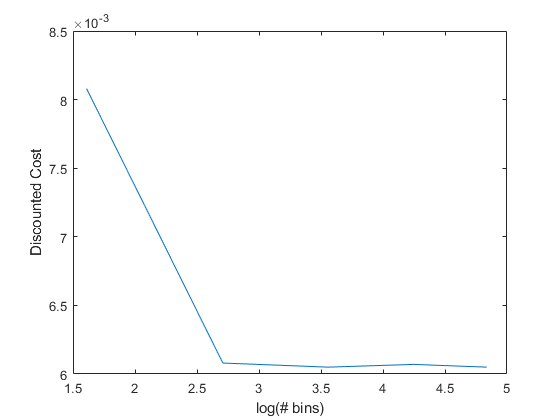
\includegraphics[height=6cm, width=10cm]{cost_5.png}
    \caption{Long-term discounted cost of learned policies}
\end{figure}

\begin{figure}[H]
    \centering
    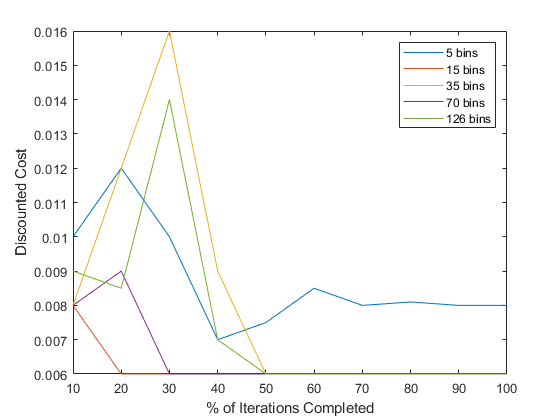
\includegraphics[height=6cm, width=10cm]{convergence_5.png}
    \caption{Convergece of learned policies}
\end{figure}

Note that the quantization gains are not significant after \( n=2 \) (which corresponds to 15 bins), which indicates that this is a sufficient quantization level for a near-optimal policy.
\newpage
Similarly, for 2-cell quantizers on \( \mathbb{X} = \{1,\ldots,16\} \),

\begin{figure}[H]
    \centering
    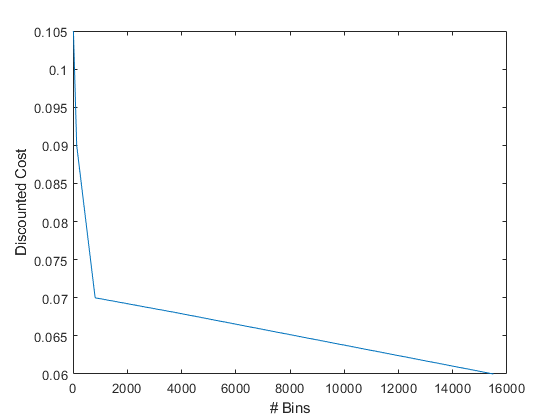
\includegraphics[height=6cm, width=10cm]{cost_16.png}
    \caption{Long-term discounted cost of learned policies}
\end{figure}

\begin{figure}[H]
    \centering
    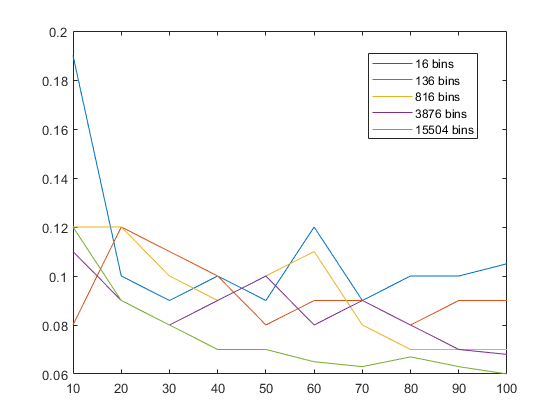
\includegraphics[height=6cm, width=10cm]{convergence_16.png}
    \caption{Convergece of learned policies}
\end{figure}

In this example, additional quantization may be required to get closer to the optimal policy.

\subsection{Comparison to Lloyd-Max Quantizer}
In these simulations, we plot the distortion for different values of \( n \) and for different quantizer rates (i.e. different sizes of \(\mathcal{M}\)). We also plot the comparison with a Lloyd-Max quantizer (another common algorithm to find an optimal quantizer), and note that our algorithm results in a lower discounted cost. We use the source alphabet \( \mathbb{X} = \{1,\ldots,13\} \), and the rate is calculated by \(\log_2(|\mathcal{M}|)\).

\begin{figure}[H]
    \centering
    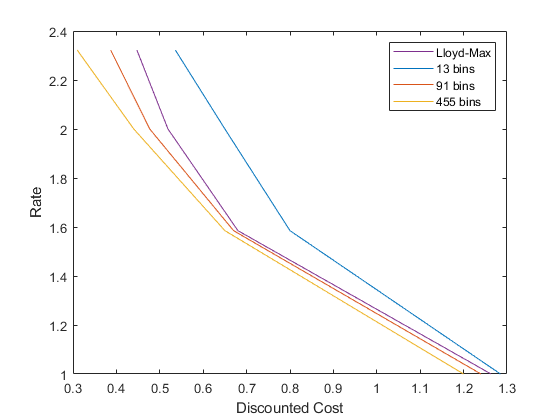
\includegraphics[height=6cm, width=10cm]{rate_distortion_lloydmax.png}
    \caption{Comparison with Lloyd-Max in Markov case}
\end{figure}

Note that for coarse quantizations, a Lloyd-Max quantizer may perform better, but as we increase the quantization, the Q-learning approach gives a lower distortion for a given rate.

Finally, we also note that our algorithm matches very closely with a Lloyd-Max quantizer in the case where the source is i.i.d., as can be seen below. Note that in this case, the Q-learning algorithm only visits one state (the one given by quantizing the distribution of \(X_0\)), and hence raising \(n\) provides no performance gain. Here we use \( \mathbb{X} = \{1,\ldots,8\} \).

\begin{figure}[H]
    \centering
    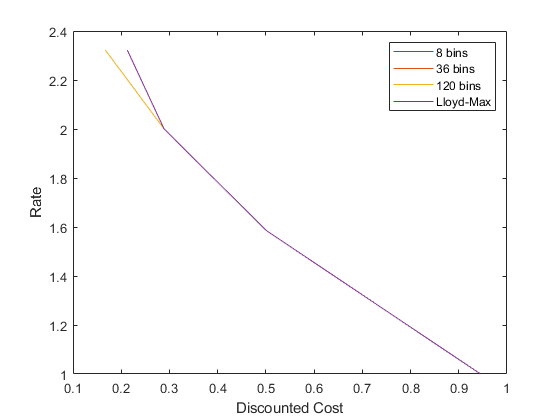
\includegraphics[height=6cm, width=10cm]{lloydmax_scalar.png}
    \caption{Comparison with Lloyd-Max in i.i.d. case}
\end{figure}

We now remark on the algorithm performance and feasibility:

\vspace{1em}
\noindent\emph{Remark 3.}\label{remark:3}
\begin{enumerate}
    \item As previously mentioned, the number of bins grows quickly with \(n\), and so running the algorithm with high \(n\) requires high amounts of memory in order to store a large Q-table. However, the number of actual visited \(\hat{\pi}_t\) tends to be much lower than the total number of bins, and so it may be possible to increase the efficiency of this algorithm by quantizing \( \pi_t \) in a non-uniform fashion (the results from~\cite{Kara} used for convergence of the algorithm allow a non-uniform quantization).
    \item As the number of bins grows, the time for the algorithm to converge becomes much higher, since it must visit more states. One must trade much longer algorithm runtime for potential performance increases. Also, since  we only have weak continuity of the transition kernel for \(\{\pi_t\}\), we do not have a bound on what quantization level we need to obtain a given performance (results from~\cite{Kara} provide these bounds under stronger notions of continuity). Therefore it is somewhat trial-and-error to find the appropriate quantization level for a given application.
    \item As mentioned in Section~\ref{section:optimal quantizers}, \(\{\pi_t\}\) updates in a Markovian fashion, and so we do not need to store the previous values of \(\pi_t\). Futhermore, from Section~\ref{section:unique-ergodicity} we have that the process \(\{\pi_t\}\) is stable (i.e. it ``forgets'' an incorrect prior) under the random exploration policy used in learning. Therefore we do not need to worry about errors accumulating over time, and in fact we can start the algorithm from any distribution \(\pi_0\) (the choice to initialize to the stationary distribution in \textbf{Algorithm 2} is just for convenience).
\end{enumerate}

\section{Future Work}
We note that the above Q-learning algorithm only converges when \( \beta \in (0,1) \) (i.e.\ for the discounted cost problem) and therefore is not applicable for the average cost problem, which is generally what we are interested in for source coding. It may be possible to adapt the Q-learning algorithm to solve the average cost problem (see e.g. \cite{Abounadi}), but this would require an extension of the results in~\cite{Kara} to this algorithm, which may require additional constraints on the source \( \mathbb{X} \). Nevertheless, we can obtain a good approximation to the average cost problem by taking \(\beta\) to be close enough to 1 (such an approach is called the ``vanishing discount'' method, see e.g.~\cite[Chapter 5]{Lerma})

Furthermore, we would like to extend the algorithm to the case when \( \mathbb{X} \) is continuous. The primary obstable here would be that the number of possible quantizers is infinite, and so a method of quantizing the space of quantizers would need to be developed. We note however that quantizing the action space (in this context, the set of quantizers) is considered in the results from~\cite{Kara}, and also all of the predictor stability/unique invariance arguments in Section~\ref{section:unique-ergodicity} hold when \( \mathbb{X} \) is continuous. So with some minor alterations, the algorithm will still converge in the continuous case.

Finally, we wish to consider the case when the channel over which \(q_t\) is sent is noisy. While most of the results from Section~\ref{section:optimal quantizers} carry over in this case, additional considerations will have to be taken in other sections (e.g. in proving uniqueness of the invariant measure).

\newpage
\printbibliography
\end{document} %chktex 17